% \section{Resultados}

% Nesta seção, são apresentadas comparações entre as três políticas de navegação descritas anteriormente: passiva, \textit{greed} e \textit{simulated annealing}. Nas simulações, o VANT percorre uma trajetória sistemática sobre a área de interesse (AI), sendo redirecionado dinamicamente de acordo com a política adotada a cada passo, conforme os alvos detectados.

% \subsection{Valores de Entrada}

% Os valores utilizados no modelo são:

% \begin{itemize}
%     \item Tamanho da AI: $300 \times 300$ milhas náuticas (MN)
%     \item Velocidade do VANT: 300 nós (MN / hora)
%     \item Alcance do radar (detecção): 50 MN
%     \item Alcance da câmera (inspeção): 20 MN
%     \item Autonomia: 2400 MN
%     \item Número de navios na AI: 10, 25, 50, 75, 100, 125, 150, 175, 200.
%     \item Distribuição espacial dos navios: uniformente aleatória.
%     \item Velocidade dos navios: parados, para simplificar a análise.
% \end{itemize}

% Os parâmetros utilizados especificamente na política de \textit{Simulated Annealing} são:

% \begin{itemize}
%     \item Temperatura inicial $T_0$: 10.0
%     \item Temperatura mínima $T_{\text{min}}$: $10^{-4}$
%     \item Fator de resfriamento $\beta$: 0.90
%     \item Número de perturbações por temperatura: 50
% \end{itemize}

% Para cada combinação de parâmetros, os experimentos são repetidos sobre 100 instâncias geradas aleatoriamente, o que totaliza $3 \times 9 \times 100 = 2700$ simulações. Os resultados são agregados por média e as métricas são apresentadas em valores absolutos (como distância percorrida e tempo de execução) ou normalizados em percentual (como proporção de navios detectados ou inspecionados), conforme apropriado para a análise.

\section{Resultados}

Nesta seção, comparam-se as políticas de navegação passiva, \textit{greed} e \textit{simulated annealing}, com base em simulações onde o VANT percorre uma trajetória sistemática sobre a área de interesse (AI), sendo redirecionado conforme a política adotada e os alvos detectados.

\subsection{Valores de Entrada}

As simulações consideram os seguintes parâmetros:

\begin{itemize}
    \item Área de interesse: $300 \times 300$ MN
    \item Velocidade do VANT: 300 nós
    \item Alcance dos sensores: radar (50 MN), câmera (20 MN)
    \item Autonomia do VANT: 2400 MN
    \item Quantidade de navios: 10 a 200 (incrementos de 25)
    \item Distribuição dos navios: aleatória e estática
\end{itemize}

Parâmetros específicos do \textit{Simulated Annealing}:

\begin{itemize}
    \item $T_0 = 10.0$, $T_{\text{min}} = 10^{-4}$
    \item Fator de resfriamento: $\beta = 0.90$
    \item Iretaçoes por ciclo: $N=50$
\end{itemize}

Cada cenário é repetido 100 vezes para as 3 políticas e 9 níveis de densidade, totalizando 2700 simulações. Os resultados são apresentados como médias, em valores absolutos (ex: distância e tempo) ou percentuais (ex: taxa de detecção/inspeção), conforme o caso.

% \subsection{Ambiente de simulação}

% A simulação foi implementada de forma modular, com dois componentes principais: o módulo \texttt{AmbienteMaritimo}, responsável por representar o cenário de patrulha e gerar os navios de forma aleatória, e o módulo \texttt{VANT}, que modela o comportamento da aeronave, incluindo sua trajetória, sensores e política de navegação. A separação entre ambiente e agente permite encapsular responsabilidades e facilita a extensão da lógica de simulação.

% A cada passo da simulação, o VANT executa um ciclo que envolve duas ações principais: movimentação e varredura sensorial. Primeiro, o VANT avança em direção ao próximo ponto definido pela sua política de navegação, respeitando sua velocidade e intervalo de tempo configurado, sem considerar a dinâmica da aeronave. A lógica de movimentação leva em conta a autonomia da aeronave: se o deslocamento planejado excede a distância restante permitida, a simulação é encerrada. 

% Após o deslocamento, o VANT verifica a presença de navios dentro de dois raios distintos: o do radar (detecção inicial) e o da câmera (inspeção visual). Os estados dos navios são atualizados conforme sua proximidade com o VANT: de \textit{nao\_detectado} para \textit{detectado} quando entram no alcance do radar, e de \textit{detectado} para \textit{inspecionado} quando também estão no raio da câmera.

% A política de navegação — \textit{passiva}, \textit{greed} ou \textit{Simulated Annealing} — define como os pontos a serem visitados são selecionados e ordenados. A \textit{passiva} segue uma rota fixa baseada em linhas paralelas; a \textit{greed} reordena os pontos (navios detectados e waypoints remanescentes) por proximidade ao VANT; e a \textit{Simulated Annealing} aplica uma metaheurística para minimizar a distância total do percurso. A política é avaliada e aplicada dinamicamente a cada passo, permitindo que o VANT adapte seu trajeto de forma progressiva conforme novos navios são detectados.

\subsection{Ambiente de Simulação}

A simulação foi implementada com dois módulos principais: \texttt{AmbienteMaritimo}, que gera o cenário e os navios aleatoriamente, e \texttt{VANT}, que modela a trajetória, sensores e política de navegação da aeronave. Essa separação facilita a manutenção e extensibilidade do sistema.

A cada passo, o VANT realiza duas ações: movimenta-se em direção ao próximo ponto definido pela política de navegação (respeitando sua velocidade e autonomia), e executa a varredura sensorial. Se o deslocamento previsto exceder a autonomia restante, a simulação é encerrada.

Em seguida, o VANT verifica a presença de navios nos raios do radar (50 MN) e da câmera (20 MN). O estado de um navio é atualizado de \textit{nao\_detectado} para \textit{detectado} ao entrar no alcance do radar, e para \textit{inspecionado} quando também estiver ao alcance da câmera.

A política de navegação define como os pontos (navios detectados e waypoints remanescentes) são ordenados. A política \textit{passiva} segue a rota fixa; a \textit{greed} prioriza os pontos mais próximos; e a \textit{Simulated Annealing} aplica uma metaheurística para minimizar a distância total. A política é avaliada dinamicamente, permitindo que o VANT ajuste sua rota conforme novos alvos são descobertos

% \subsection{Distância percorrida}

% A Figura~\ref{fig:distancia} apresenta a média da distância total percorrida pelo VANT ao longo da missão, conforme a política de navegação e a quantidade de navios. A política \textit{passiva} mantém trajetória constante, enquanto as políticas com replanejamento (\textit{greed} e \textit{Simulated Annealing}) aumentam progressivamente a distância total percorrida à medida que mais navios são introduzidos no cenário.

% \begin{figure}[H]
%     \centering
%     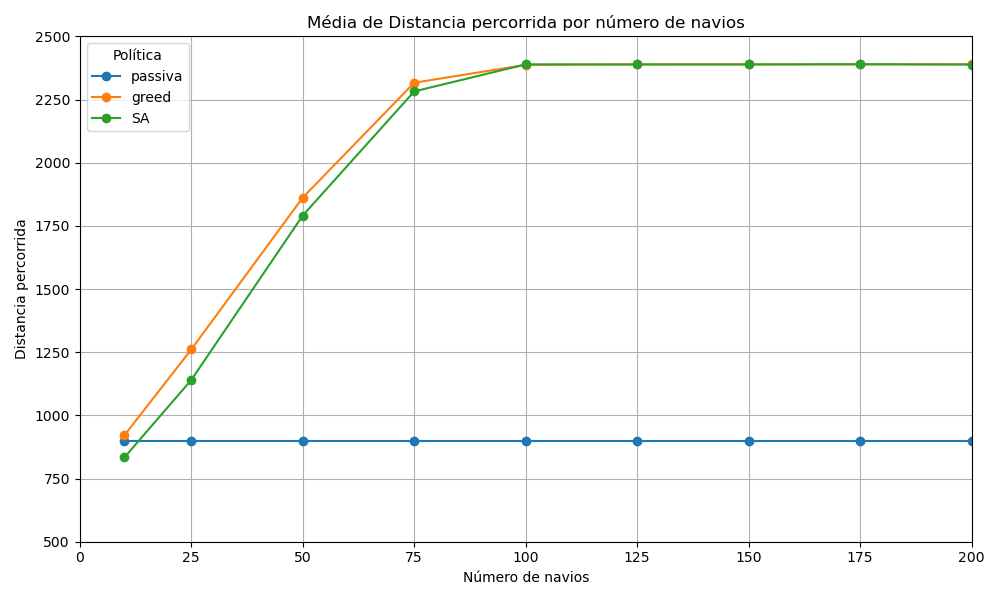
\includegraphics[width=0.7\textwidth]{fig/resultado_dis.png}
%     \caption{Média da distância percorrida por política e quantidade de navios.}
%     \label{fig:distancia}
% \end{figure}


% Observa-se que tanto a política \textit{greed} quanto a de \textit{Simulated Annealing} saturam a curva, atingindo a autonomia máxima do VANT a partir de 100 navios. Antes desse ponto de saturação, a política \textit{Simulated Annealing} percorre uma distância média menor do que a \textit{greed}, indicando que o método está encontrando soluções mais eficientes em termos de distância total percorrida.

\subsection{Distância Percorrida}

A Figura~\ref{fig:distancia} mostra a média da distância total percorrida pelo VANT conforme a política de navegação e a quantidade de navios. A política \textit{passiva} mantém uma trajetória fixa, enquanto \textit{greed} e \textit{Simulated Annealing} aumentam a distância percorrida à medida que mais navios são introduzidos.

\begin{figure}[H]
    \centering
    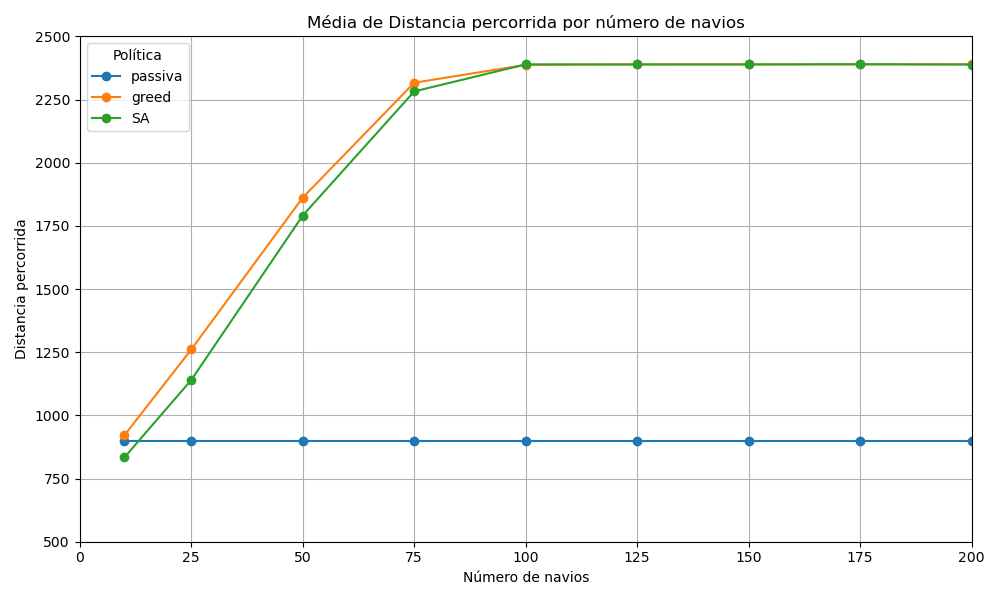
\includegraphics[width=0.7\textwidth]{fig/resultado_dis.png}
    \caption{Média da distância percorrida por política e quantidade de navios.}
    \label{fig:distancia}
\end{figure}

A partir de 100 navios, ambas as políticas ativas atingem o limite de autonomia do VANT. Antes disso, \textit{Simulated Annealing} apresenta menor distância média que \textit{greed}, indicando trajetórias mais eficientes.


% \subsection{Detecção de navios}

% A Figura~\ref{fig:detectados} mostra a média percentual de navios detectados ao longo da missão, considerando os que foram detectados ao menos uma vez, independentemente de terem sido inspecionados. A política \textit{passiva} apresenta uma taxa de detecção aproximadamente constante e, na maioria dos cenários, superior às demais políticas, exceto entre 50 e 125 navios, onde ocorre um cruzamento temporário de desempenho. Esse comportamento está relacionado ao fato de que, ao não se desviar da rota original, o VANT percorre toda a área de interesse, aumentando a probabilidade de que todos os navios dentro do alcance do radar sejam detectados.


% \begin{figure}[H]
%     \centering
%     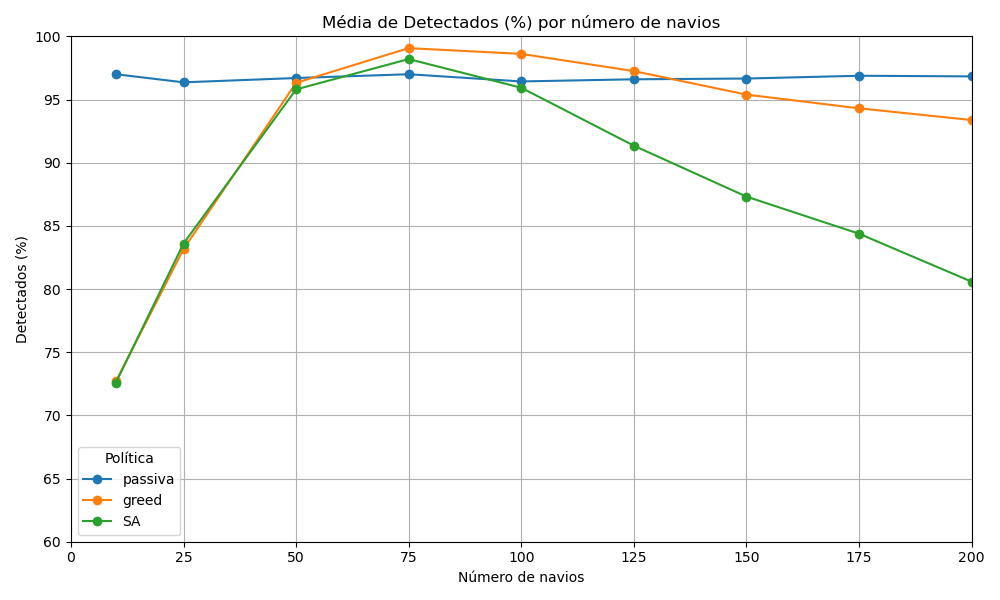
\includegraphics[width=0.7\textwidth]{fig/resultado_det.png}
%     \caption{Média percentual de navios detectados por política e quantidade de navios.}
%     \label{fig:detectados}
% \end{figure}

% As políticas \textit{greed} e \textit{Simulated Annealing} apresentam desempenho semelhante em cenários com até 75 navios. A partir de cenários mais densos, a política \textit{greed} tende a apresentar maior taxa de detecção. A queda geral no desempenho dessas duas políticas, em cenários de 100 navios em diante pode, ser associada à limitação de autonomia do VANT, conforme indicado na Figura~\ref{fig:distancia}, que mostra a saturação da distância percorrida nos cenários com maior número de navios.

\subsection{Detecção de Navios}

A Figura~\ref{fig:detectados} apresenta a média percentual de navios detectados ao longo da missão, considerando aqueles identificados pelo radar ao menos uma vez. A política \textit{passiva} mantém uma taxa de detecção quase constante e, na maioria dos cenários, superior às demais, exceto entre 50 e 125 navios, onde há um cruzamento temporário de desempenho.

\begin{figure}[H]
    \centering
    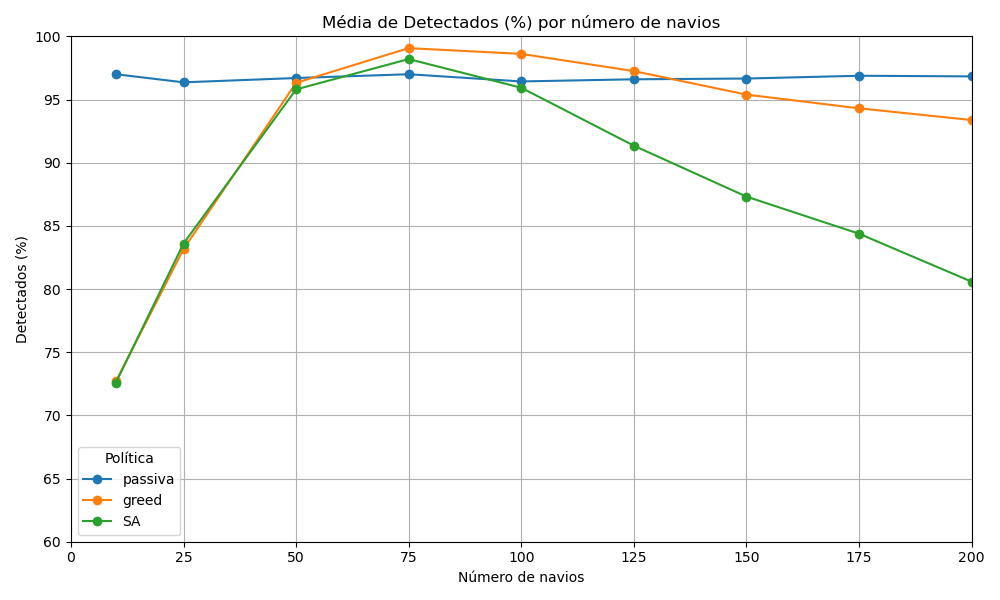
\includegraphics[width=0.7\textwidth]{fig/resultado_det.png}
    \caption{Média percentual de navios detectados por política e quantidade de navios.}
    \label{fig:detectados}
\end{figure}

Esse desempenho da política \textit{passiva} se deve ao fato de ela cobrir toda a área de interesse, maximizando as chances de detecção por radar. Já \textit{greed} e \textit{Simulated Annealing} têm desempenho similar até 75 navios, mas em cenários mais densos a \textit{greed} tende a detectar mais. A queda geral de desempenho dessas políticas a partir de 100 navios está ligada à limitação de autonomia do VANT, conforme indicado na Figura~\ref{fig:distancia}.

% \subsection{Inspeção de navios}

% A Figura~\ref{fig:inspecionados} apresenta a média percentual de navios inspecionados em função da quantidade total de navios no cenário, para cada política de navegação considerada. Observa-se que a política \textit{passiva} mantém taxas de inspeção muito inferiores às políticas \textit{greed} e \textit{Simulated Annealing} em todos os cenários, o que é esperado, já que essas políticas incluem mecanismos de desvio da rota original para inspecionar alvos detectados.

% \begin{figure}[H]
%     \centering
%     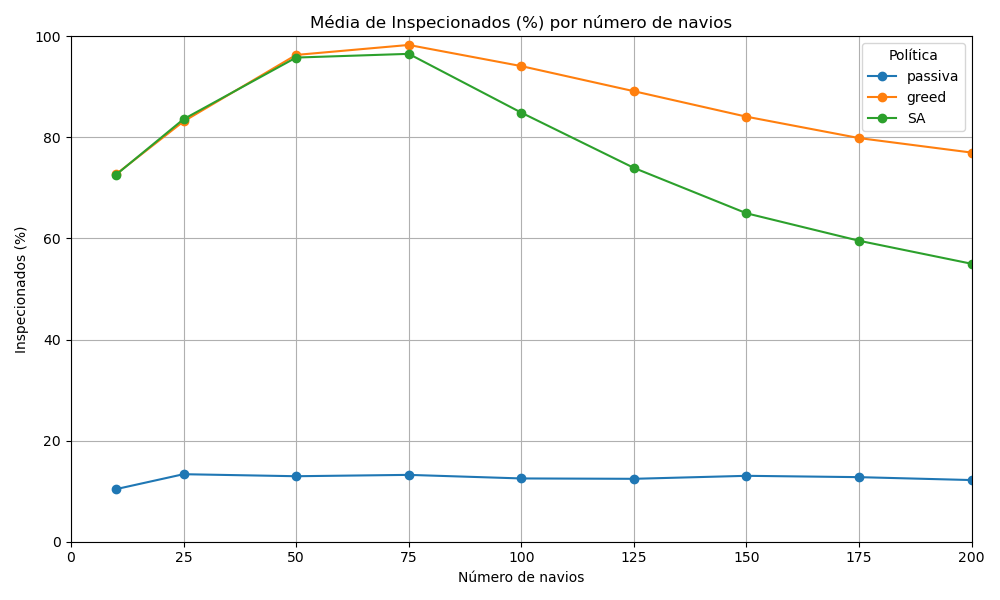
\includegraphics[width=0.7\textwidth]{fig/resultado_ins.png}
%     \caption{Média percentual de navios inspecionados por política e quantidade de navios.}
%     \label{fig:inspecionados}
% \end{figure}

% Assim como na detecção de navios, as políticas \textit{greed} e \textit{Simulated Annealing} apresentam desempenho próximo em cenários com até 75 navios. Em cenários mais densos, a política \textit{greed} tende a alcançar uma maior taxa de inspeção. A redução gradual nas taxas médias pode ser atribuída à limitação de autonomia do VANT, que, ao atingir sua capacidade máxima de voo, encerra a missão antes de completar a inspeção de todos os alvos.

\subsection{Inspeção de Navios}

A Figura~\ref{fig:inspecionados} mostra a média percentual de navios inspecionados em função da quantidade de navios no cenário. A política \textit{passiva} apresenta taxas significativamente inferiores às de \textit{greed} e \textit{Simulated Annealing}, como esperado, por não desviar da rota para confirmar alvos detectados.

\begin{figure}[H]
    \centering
    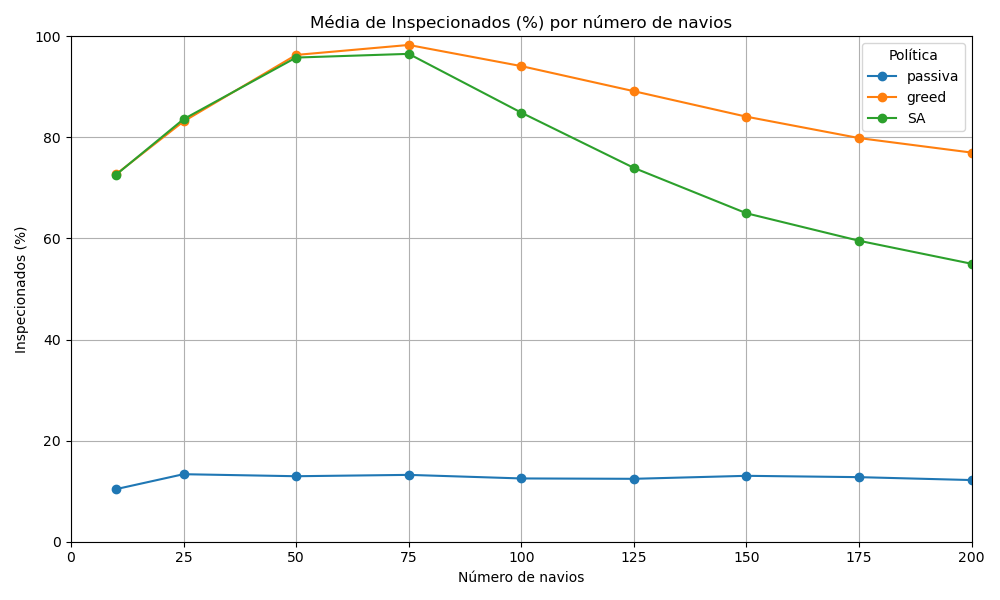
\includegraphics[width=0.7\textwidth]{fig/resultado_ins.png}
    \caption{Média percentual de navios inspecionados por política e quantidade de navios.}
    \label{fig:inspecionados}
\end{figure}

As políticas ativas têm desempenho semelhante até 75 navios. Em cenários mais densos, \textit{greed} tende a inspecionar mais. A queda nas taxas médias deve-se à limitação de autonomia do VANT, que encerra a missão antes de visitar todos os alvos.

% \subsection{Tempo de execução}

% A Figura~\ref{fig:tempo_execucao} exibe o tempo médio de execução das simulações para cada política, em função do número de navios presentes no cenário. A política \textit{Simulated Annealing} apresenta tempo crescente com o aumento do número de navios, enquanto as políticas \textit{passiva} e \textit{greed} mantêm tempos praticamente constantes e significativamente inferiores.


% \begin{figure}[H]
%     \centering
%     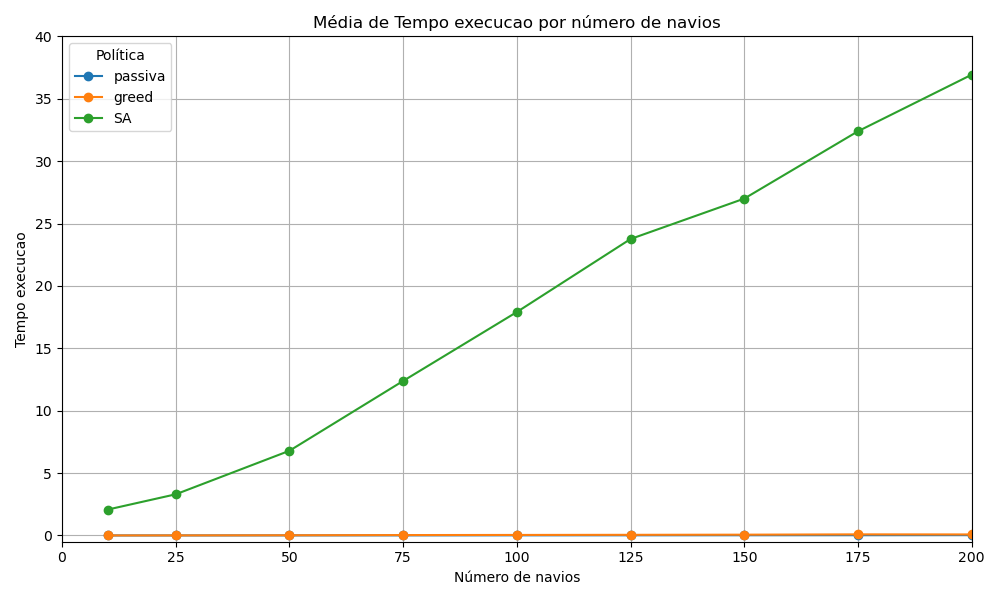
\includegraphics[width=0.7\textwidth]{fig/resultado_tem.png}
%     \caption{Tempo médio de execução da simulação por política e quantidade de navios.}
%     \label{fig:tempo_execucao}
% \end{figure}

% O número de iterações do algoritmo de \textit{Simulated Annealing} é determinado pelos parâmetros $T_0$, $T_{\text{min}}$, $\beta$ e o número de perturbações. Porém cada iteração, é calculado o custo total da rota, somando-se as distâncias entre pontos consecutivos, o que ocorre com complexidade $O(n)$, sendo $n$ o número de pontos — composto pelos \textit{waypoints} restantes e pelos navios detectados não inspecionados. Isso resulta em um tempo de execução que cresce linearmente com o número de navios no cenário.

% A política \textit{greed} também possui custo computacional associado à reordenação dos pontos relevantes. A cada passo, calcula-se a distância entre o VANT e cada ponto candidato, operação com custo $O(n)$, seguida pela ordenação desses pontos por proximidade, que tem custo $O(n \log n)$. No entanto, como essa operação ocorre apenas uma vez por passo de simulação (e não várias vezes como no \textit{Simulated Annealing}), o tempo total de execução é tão próximo de zero que aparenta ser constante, mesmo com o aumento do número de navios.

\subsection{Tempo de Execução}

A Figura~\ref{fig:tempo_execucao} mostra o tempo médio de execução das simulações para cada política, em função do número de navios no cenário. A política \textit{Simulated Annealing} apresenta tempo crescente, enquanto \textit{passiva} e \textit{greed} mantêm tempos quase constantes e significativamente menores.

\begin{figure}[H]
    \centering
    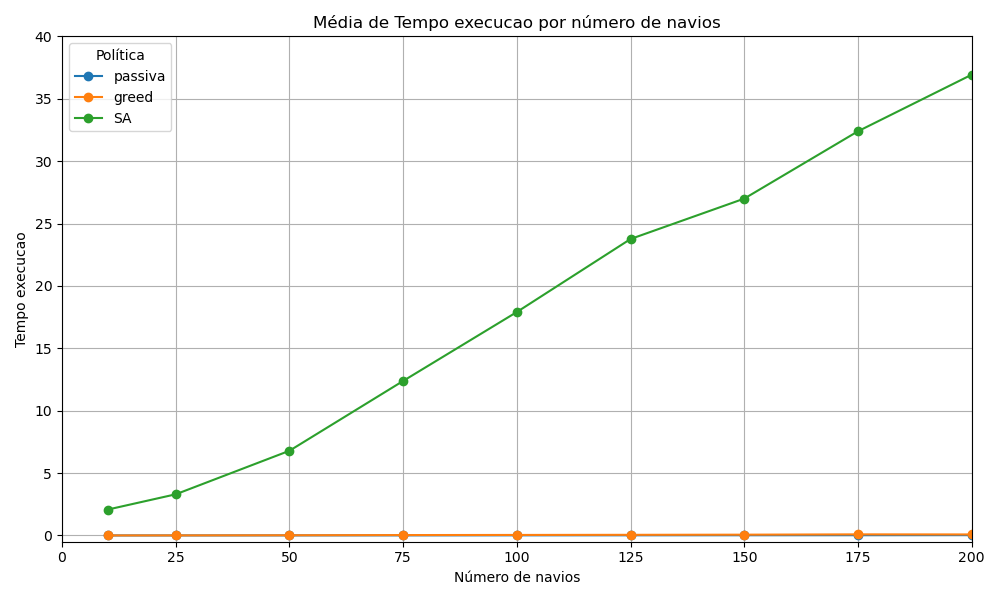
\includegraphics[width=0.7\textwidth]{fig/resultado_tem.png}
    \caption{Tempo médio de execução da simulação por política e quantidade de navios.}
    \label{fig:tempo_execucao}
\end{figure}

O tempo da política \textit{Simulated Annealing} cresce linearmente com o número de navios, pois a cada iteração (controlada por $T_0$, $T_{\text{min}}$, $\beta$ e número de perturbações), calcula-se o custo da rota com complexidade $O(n)$, onde $n$ é o total de pontos a visitar.

A política \textit{greed} também cresce linearmente, pois em cada passo calcula distâncias ($O(n)$) e ordena os candidatos ($O(n \log n)$). No entanto, os tempos absolutos são muito menores (entre 0{,}01 e 0{,}09 segundos), o que faz o gráfico aparentar comportamento constante.

% \subsection{Comparação visual das trajetórias}

% A Figura~\ref{fig:trajetorias_comparacao} apresenta os resultados das simulações com 50 navios para as três políticas de navegação implementadas: (a) \textit{passiva}, (b) \textit{greed} e (c) \textit{Simulated Annealing}. Cada subfigura exibe a rota planejada (waypoints paralelos), o caminho percorrido pelo VANT (trajetória real) e a localização dos navios inspecionados. As imagens destacam as diferenças na forma como a trajetória é ajustada durante o voo, conforme a política adotada.

% \begin{figure}[H]
%     \centering
%     \begin{subfigure}{0.4\textwidth}
%         \centering
%         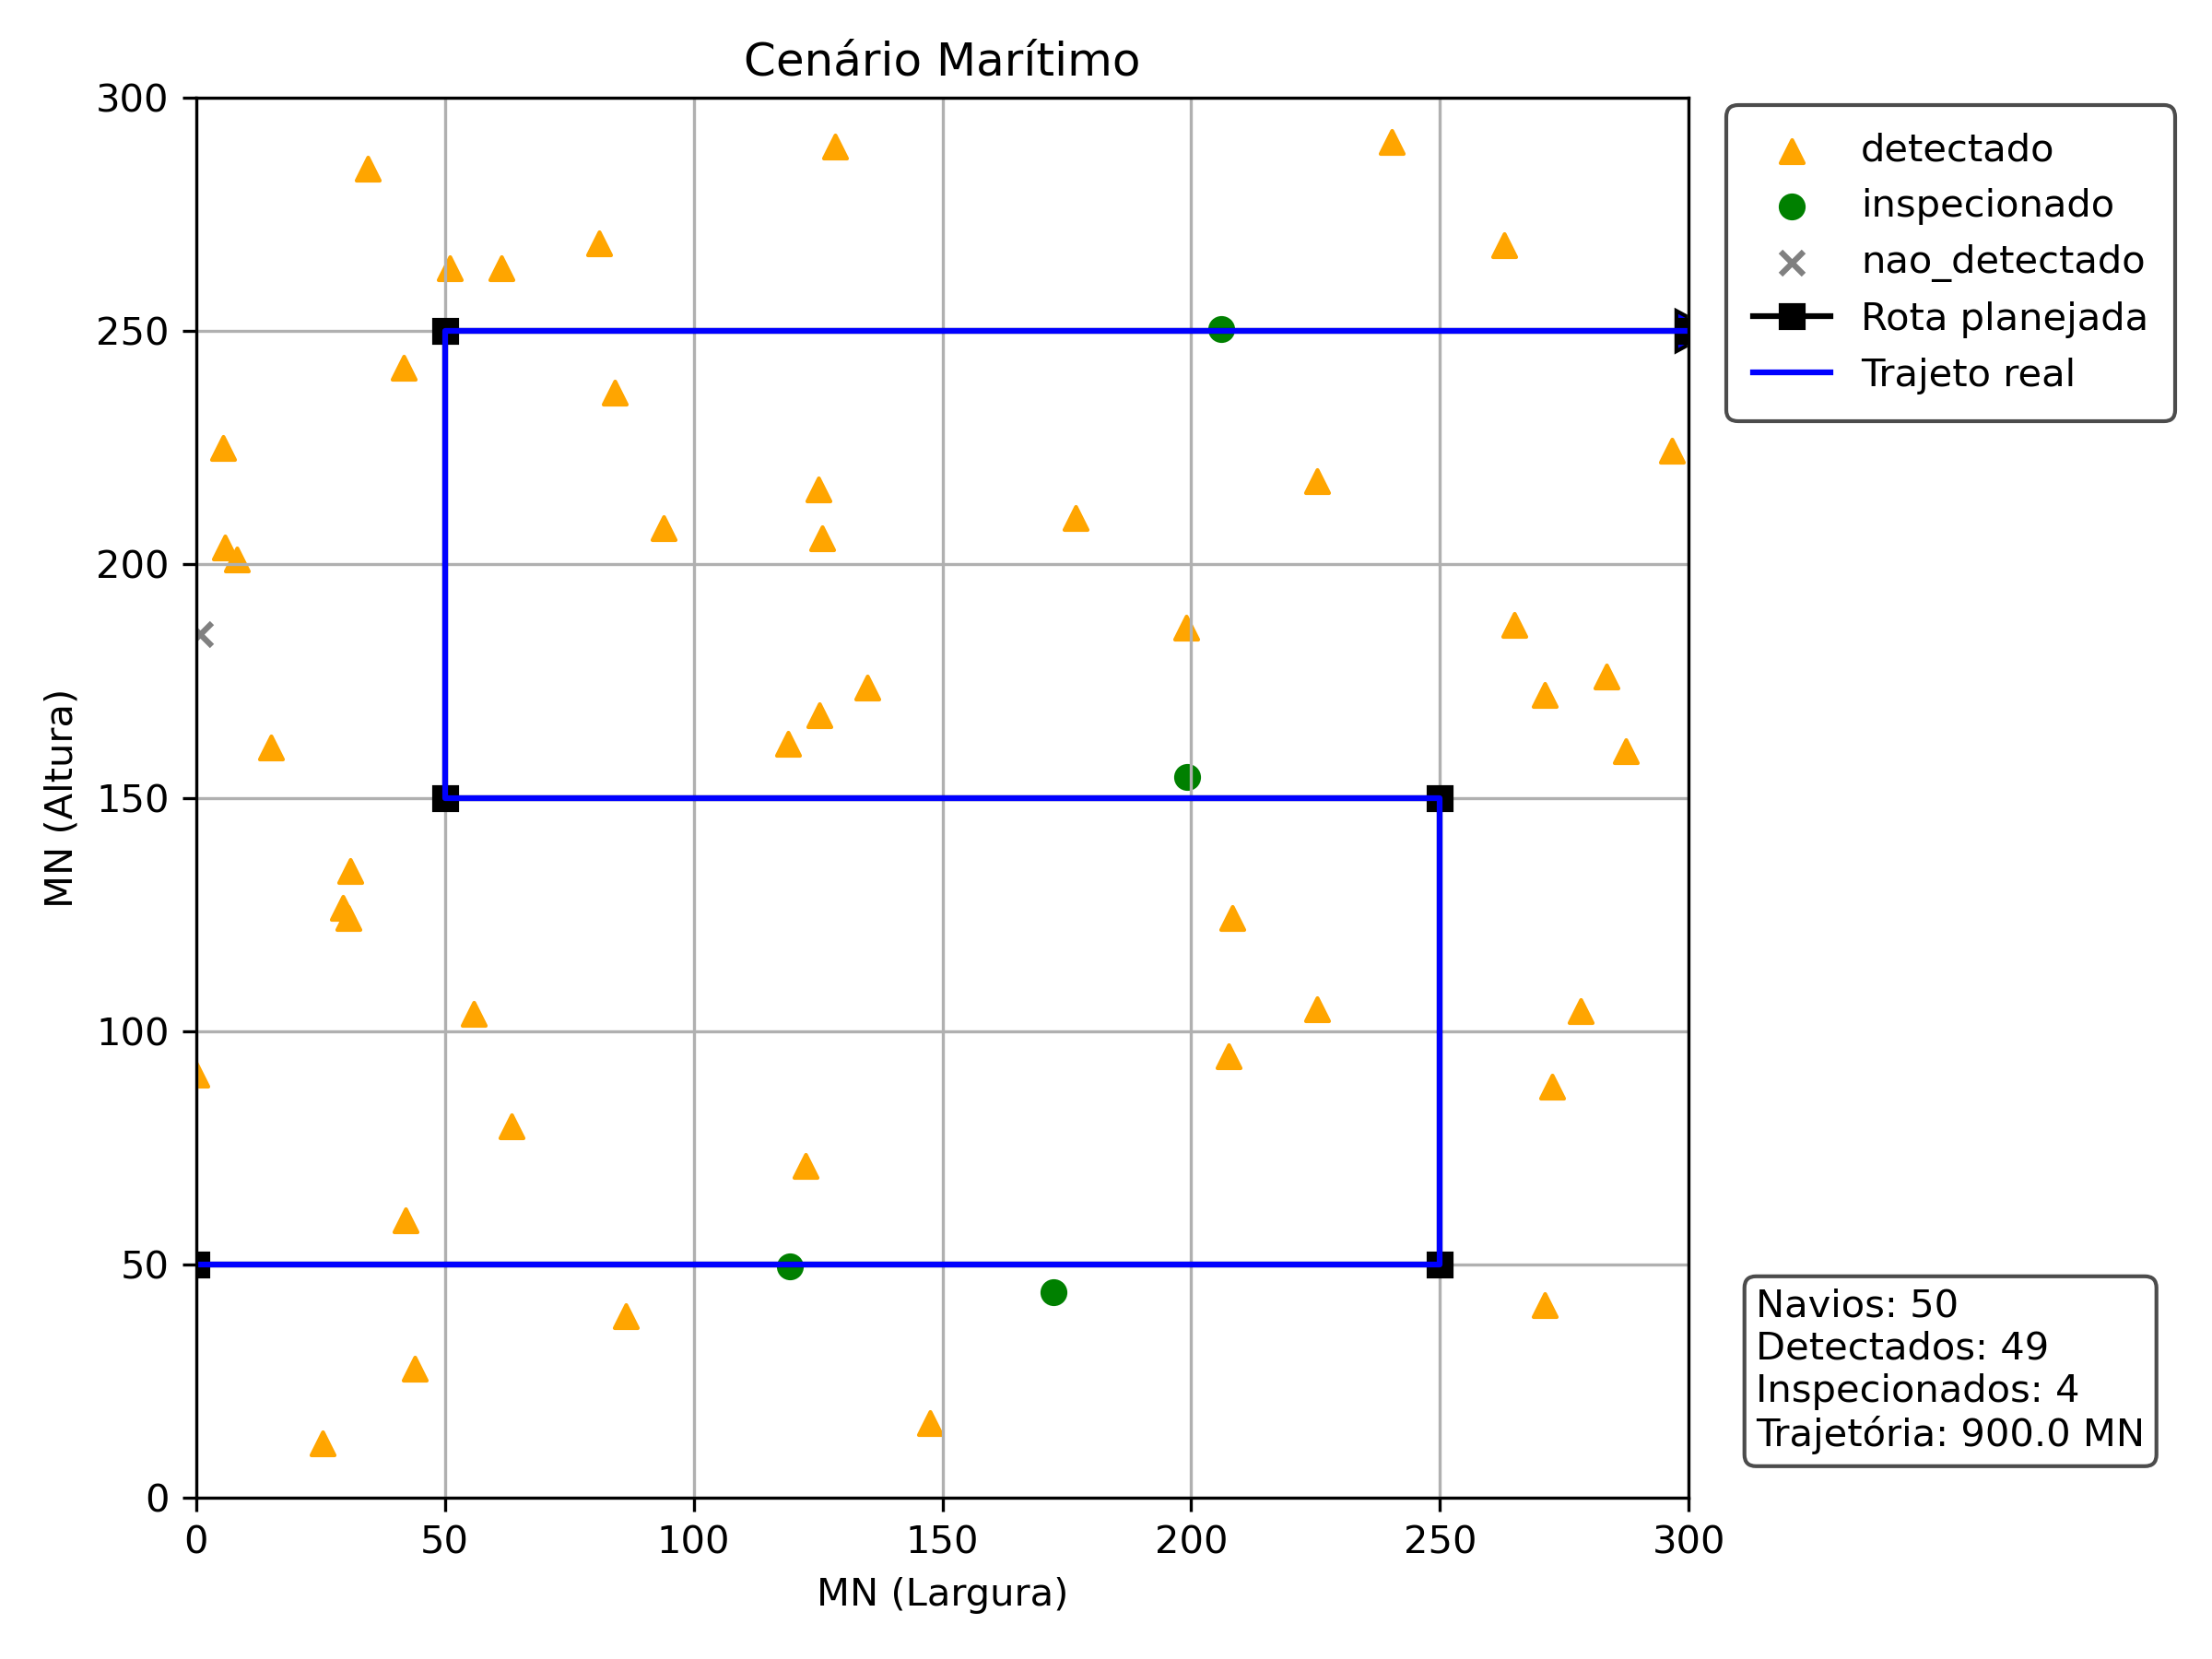
\includegraphics[width=\linewidth]{fig/passiva.png}
%         \caption{\textit{Passiva}}
%         \label{fig:trajetoria_passiva}
%     \end{subfigure}
%     \hfill
%     \begin{subfigure}{0.4\textwidth}
%         \centering
%         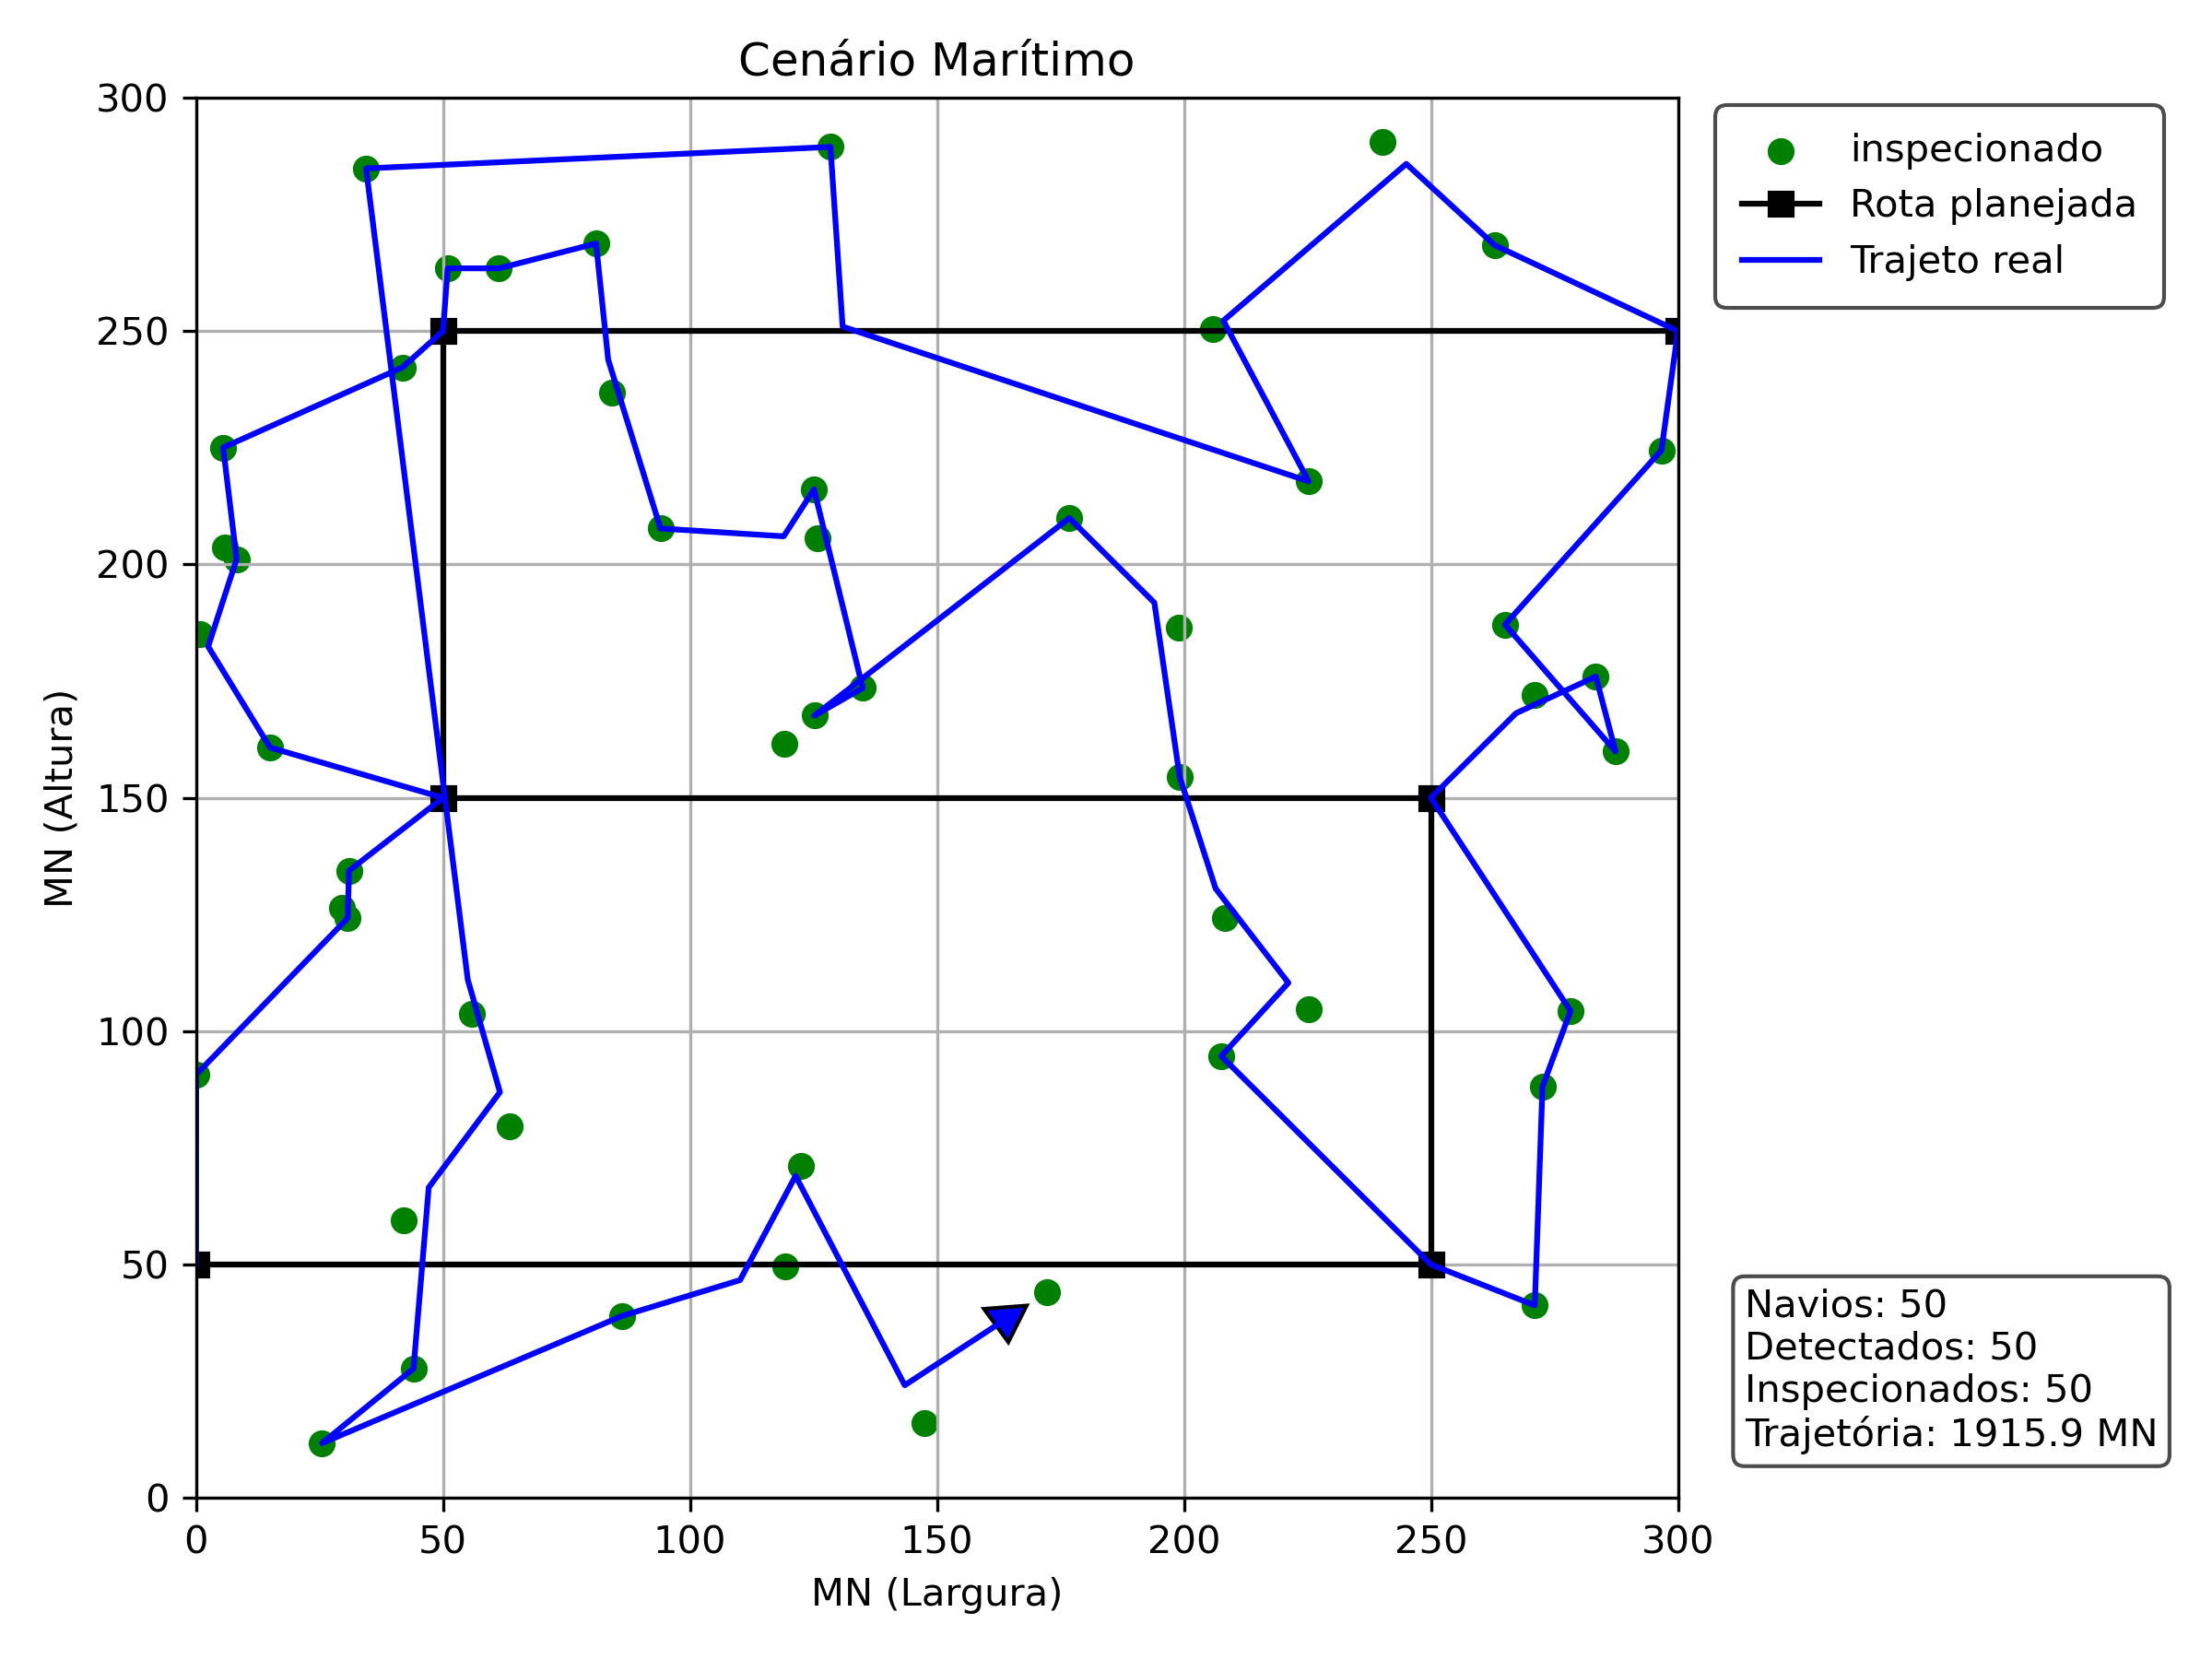
\includegraphics[width=\linewidth]{fig/greed.png}
%         \caption{\textit{Greed}}
%         \label{fig:trajetoria_greed}
%     \end{subfigure}
%     \hfill
%     \begin{subfigure}{0.4\textwidth}
%         \centering
%         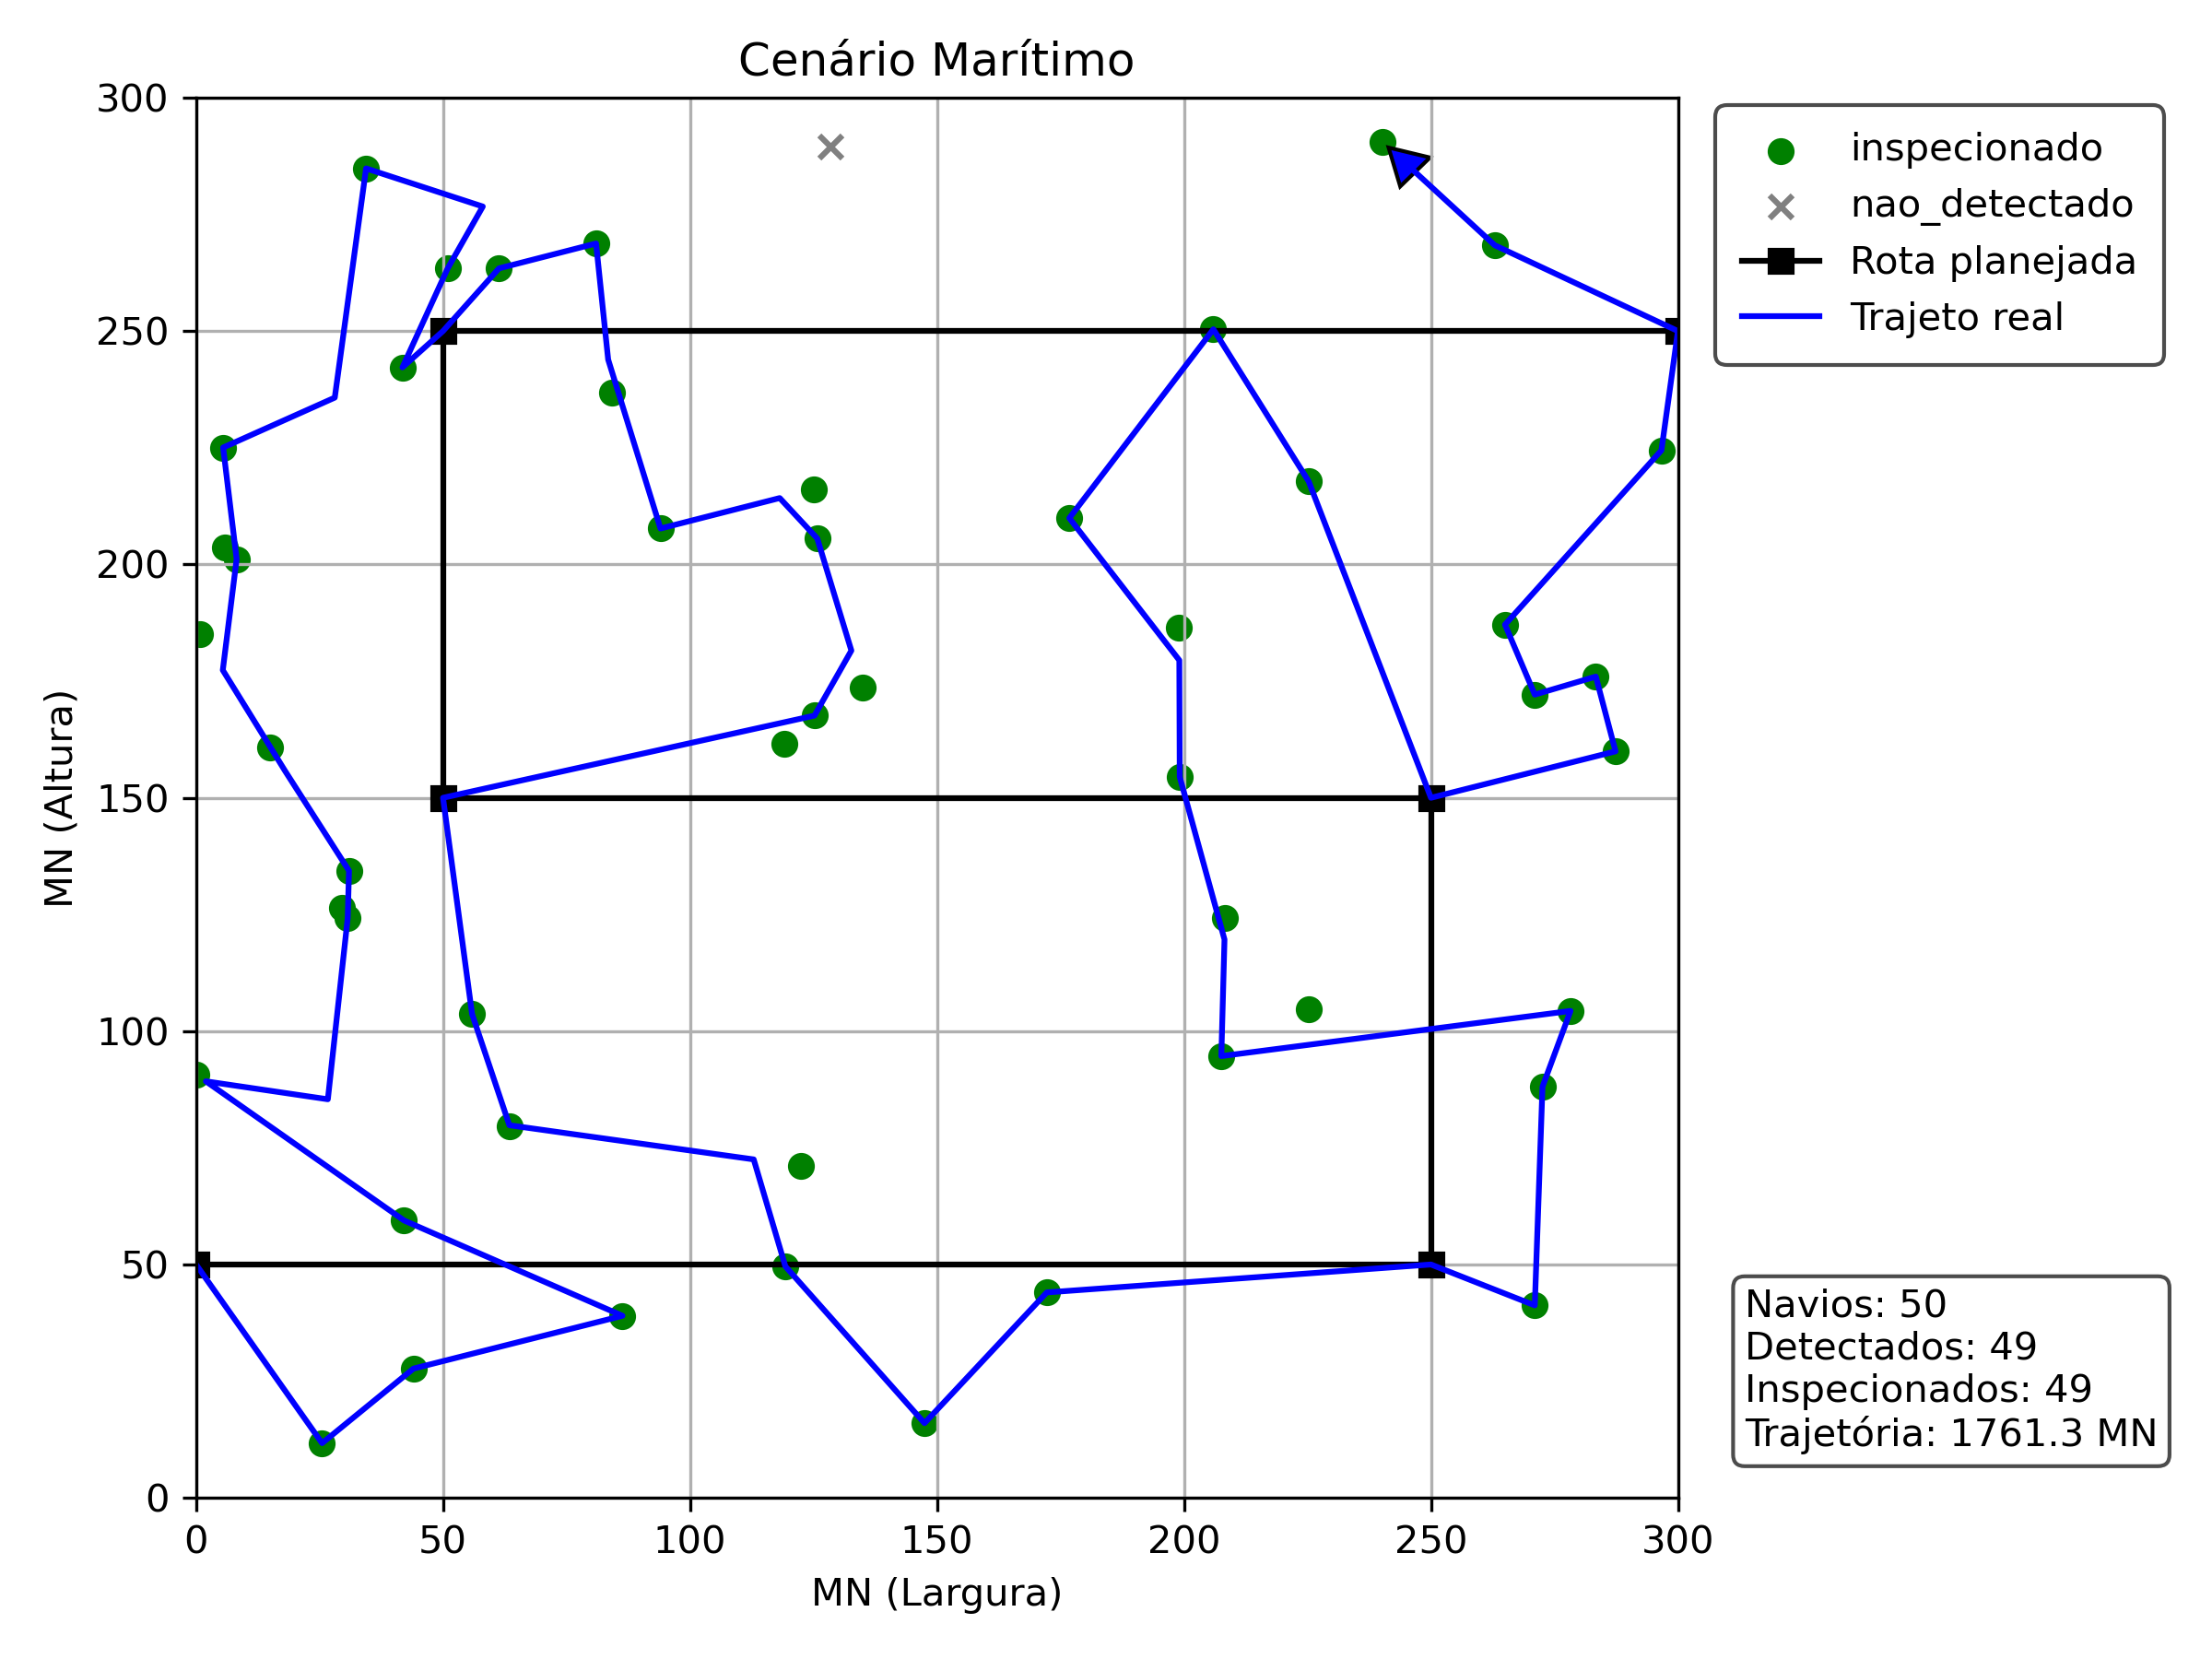
\includegraphics[width=\linewidth]{fig/SA.png}
%         \caption{\textit{Simulated Annealing}}
%         \label{fig:trajetoria_sa}
%     \end{subfigure}
%     \caption{Trajetória do VANT para as três políticas de navegação (50 navios).}
%     \label{fig:trajetorias_comparacao}
% \end{figure}

% Na política \textit{passiva}, o VANT segue a rota de referência, inspecionando os navios que encontra ao longo do caminho. Já na política \textit{greed}, o VANT desvia da rota original para inspecionar os navios mais próximos, resultando em uma trajetória mais adaptativa. Por fim, na política \textit{Simulated Annealing}, o VANT também ajusta sua trajetória, mas de forma mais otimizada, buscando minimizar a distância total percorrida. Uma diferença notável é que, na política \textit{greed}, o VANT cruza a própria trajetória algumas vezes, o que não ocorre na política \textit{Simulated Annealing}. Esse comportamento sugere que a política \textit{greed} tende a gerar trajetórias com sobreposição de caminhos, o que pode resultar em maior distância total percorrida. Em contraste, a política \textit{Simulated Annealing} evita esse tipo de cruzamento, produzindo trajetórias mais diretas.

\subsection{Comparação Visual das Trajetórias}

A Figura~\ref{fig:trajetorias_comparacao} mostra os resultados das simulações com 50 navios para as três políticas de navegação. Cada subfigura exibe os waypoints paralelos, a trajetória real do VANT e os navios inspecionados, ilustrando como cada política ajusta o percurso durante o voo.

\begin{figure}[H]
    \centering
    \begin{subfigure}{0.4\textwidth}
        \centering
        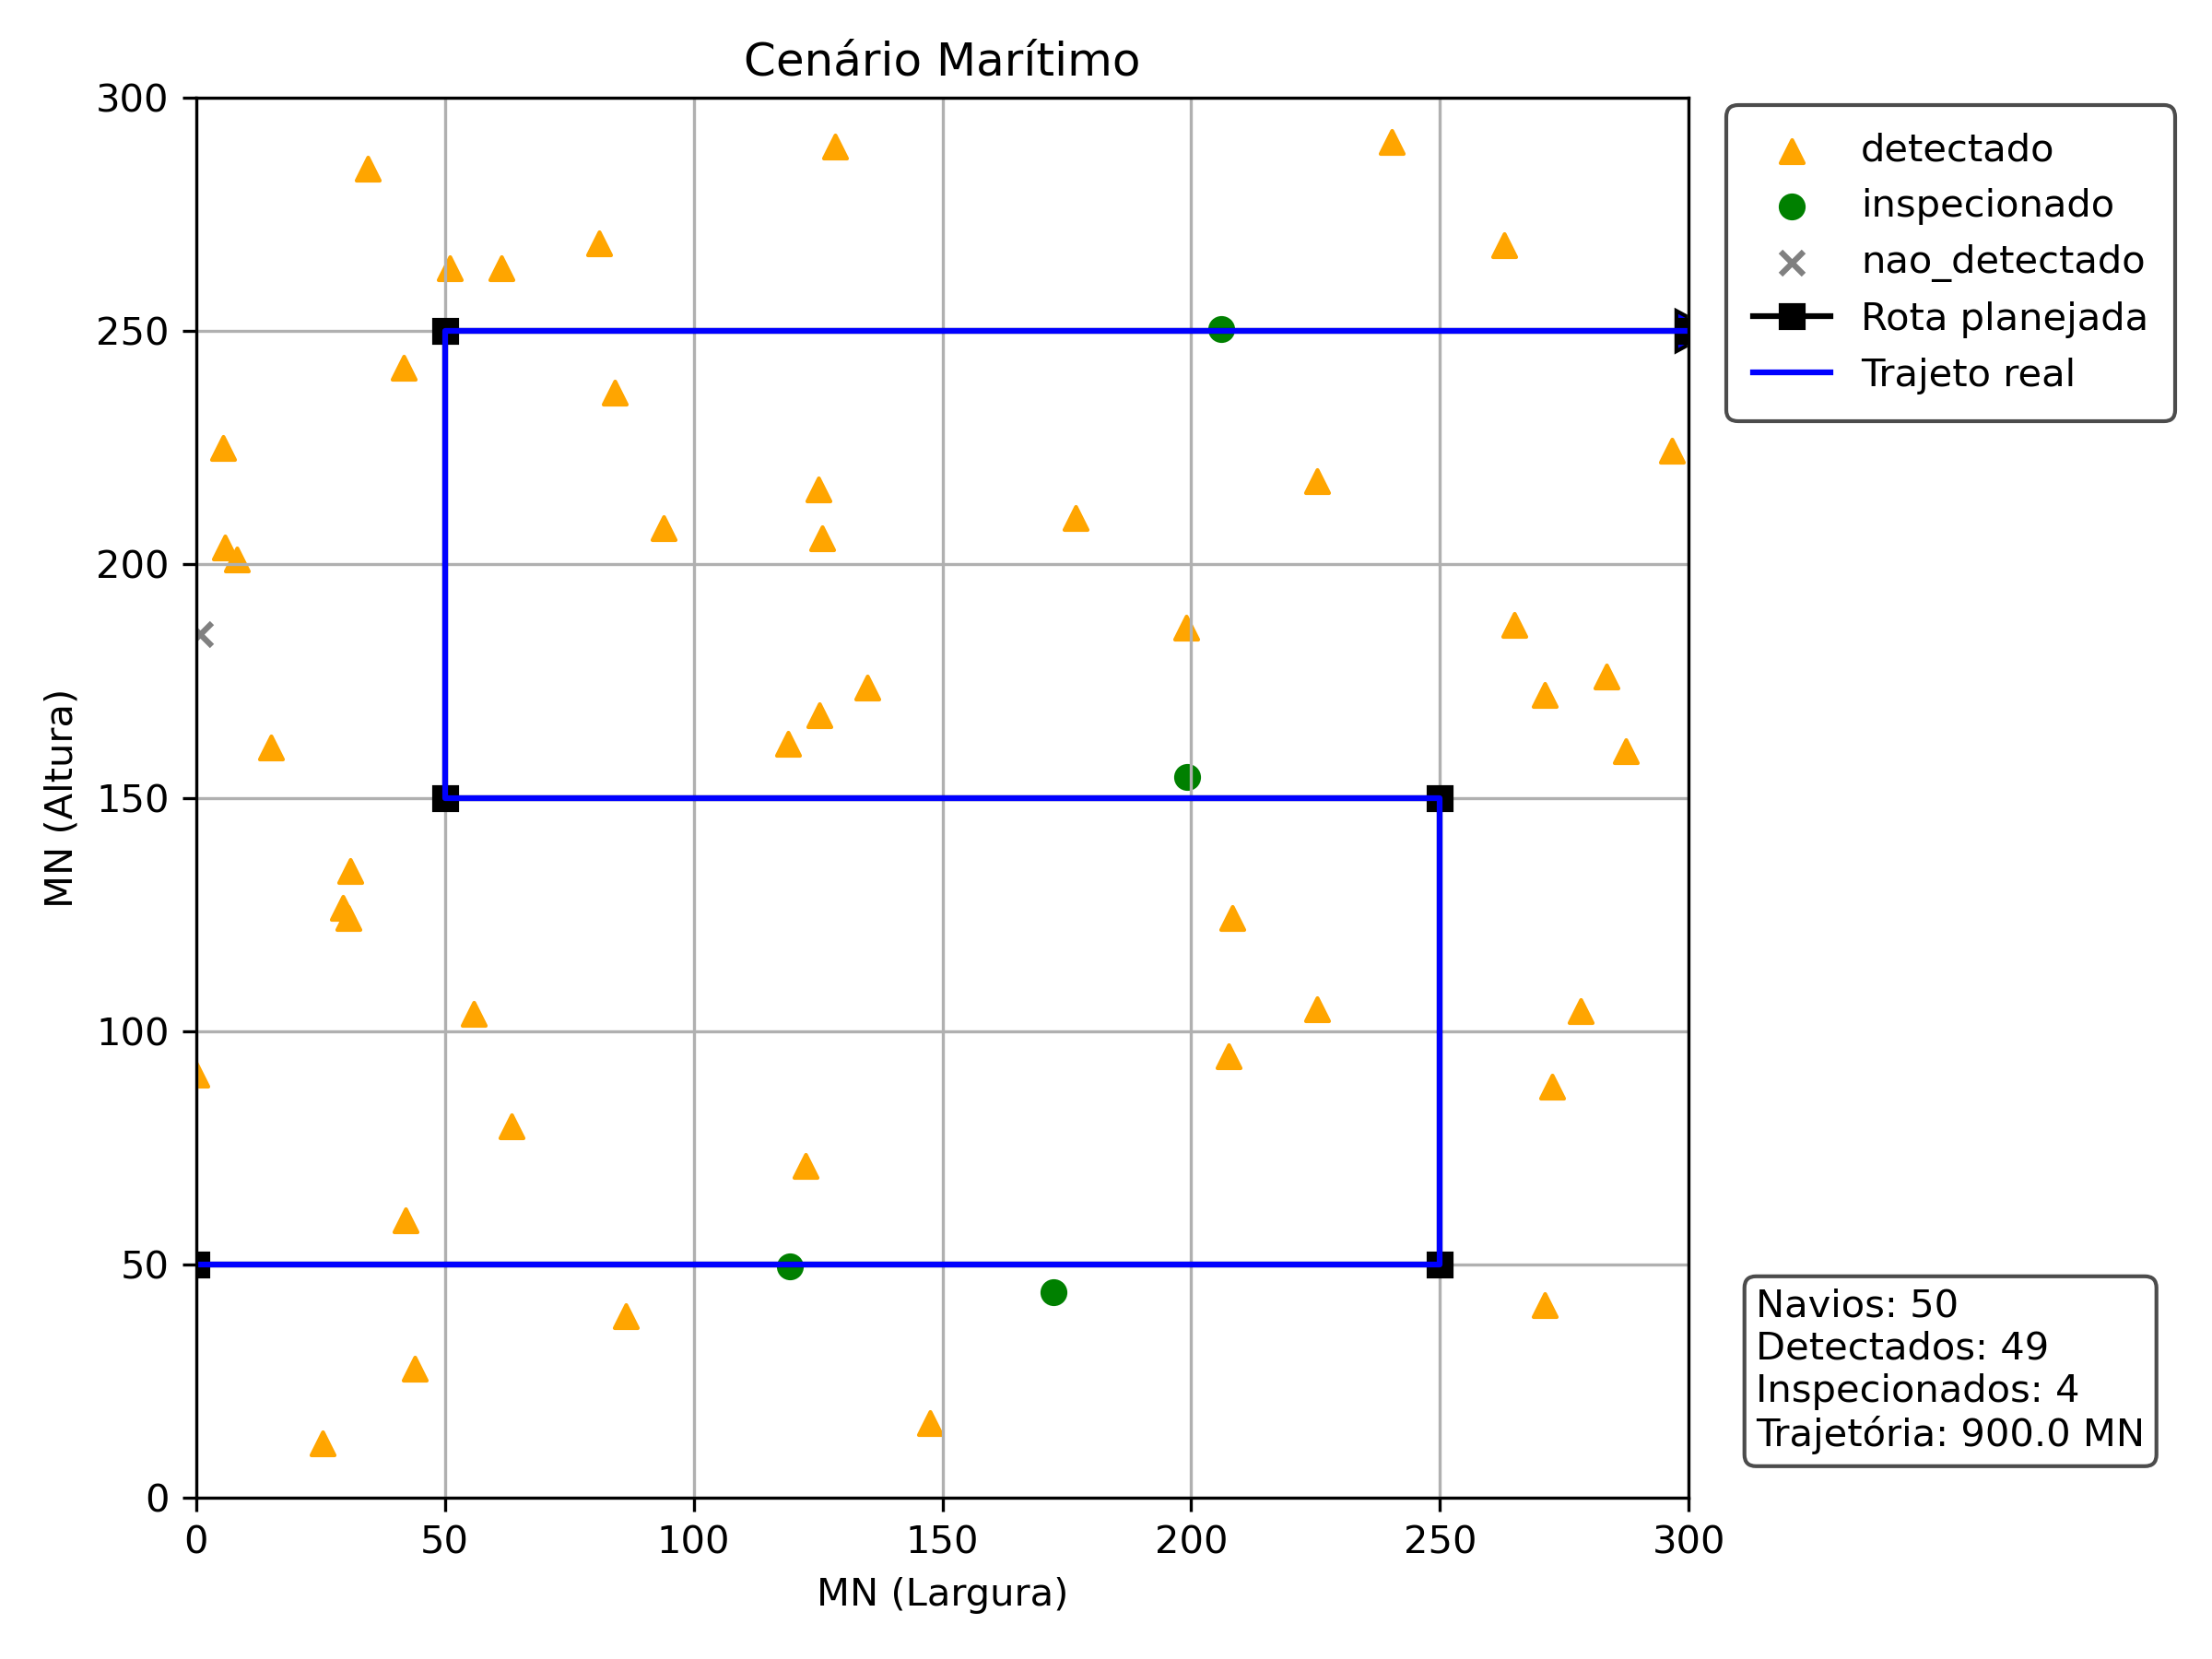
\includegraphics[width=\linewidth]{fig/passiva.png}
        \caption{\textit{Passiva}}
        \label{fig:trajetoria_passiva}
    \end{subfigure}
    \hfill
    \begin{subfigure}{0.4\textwidth}
        \centering
        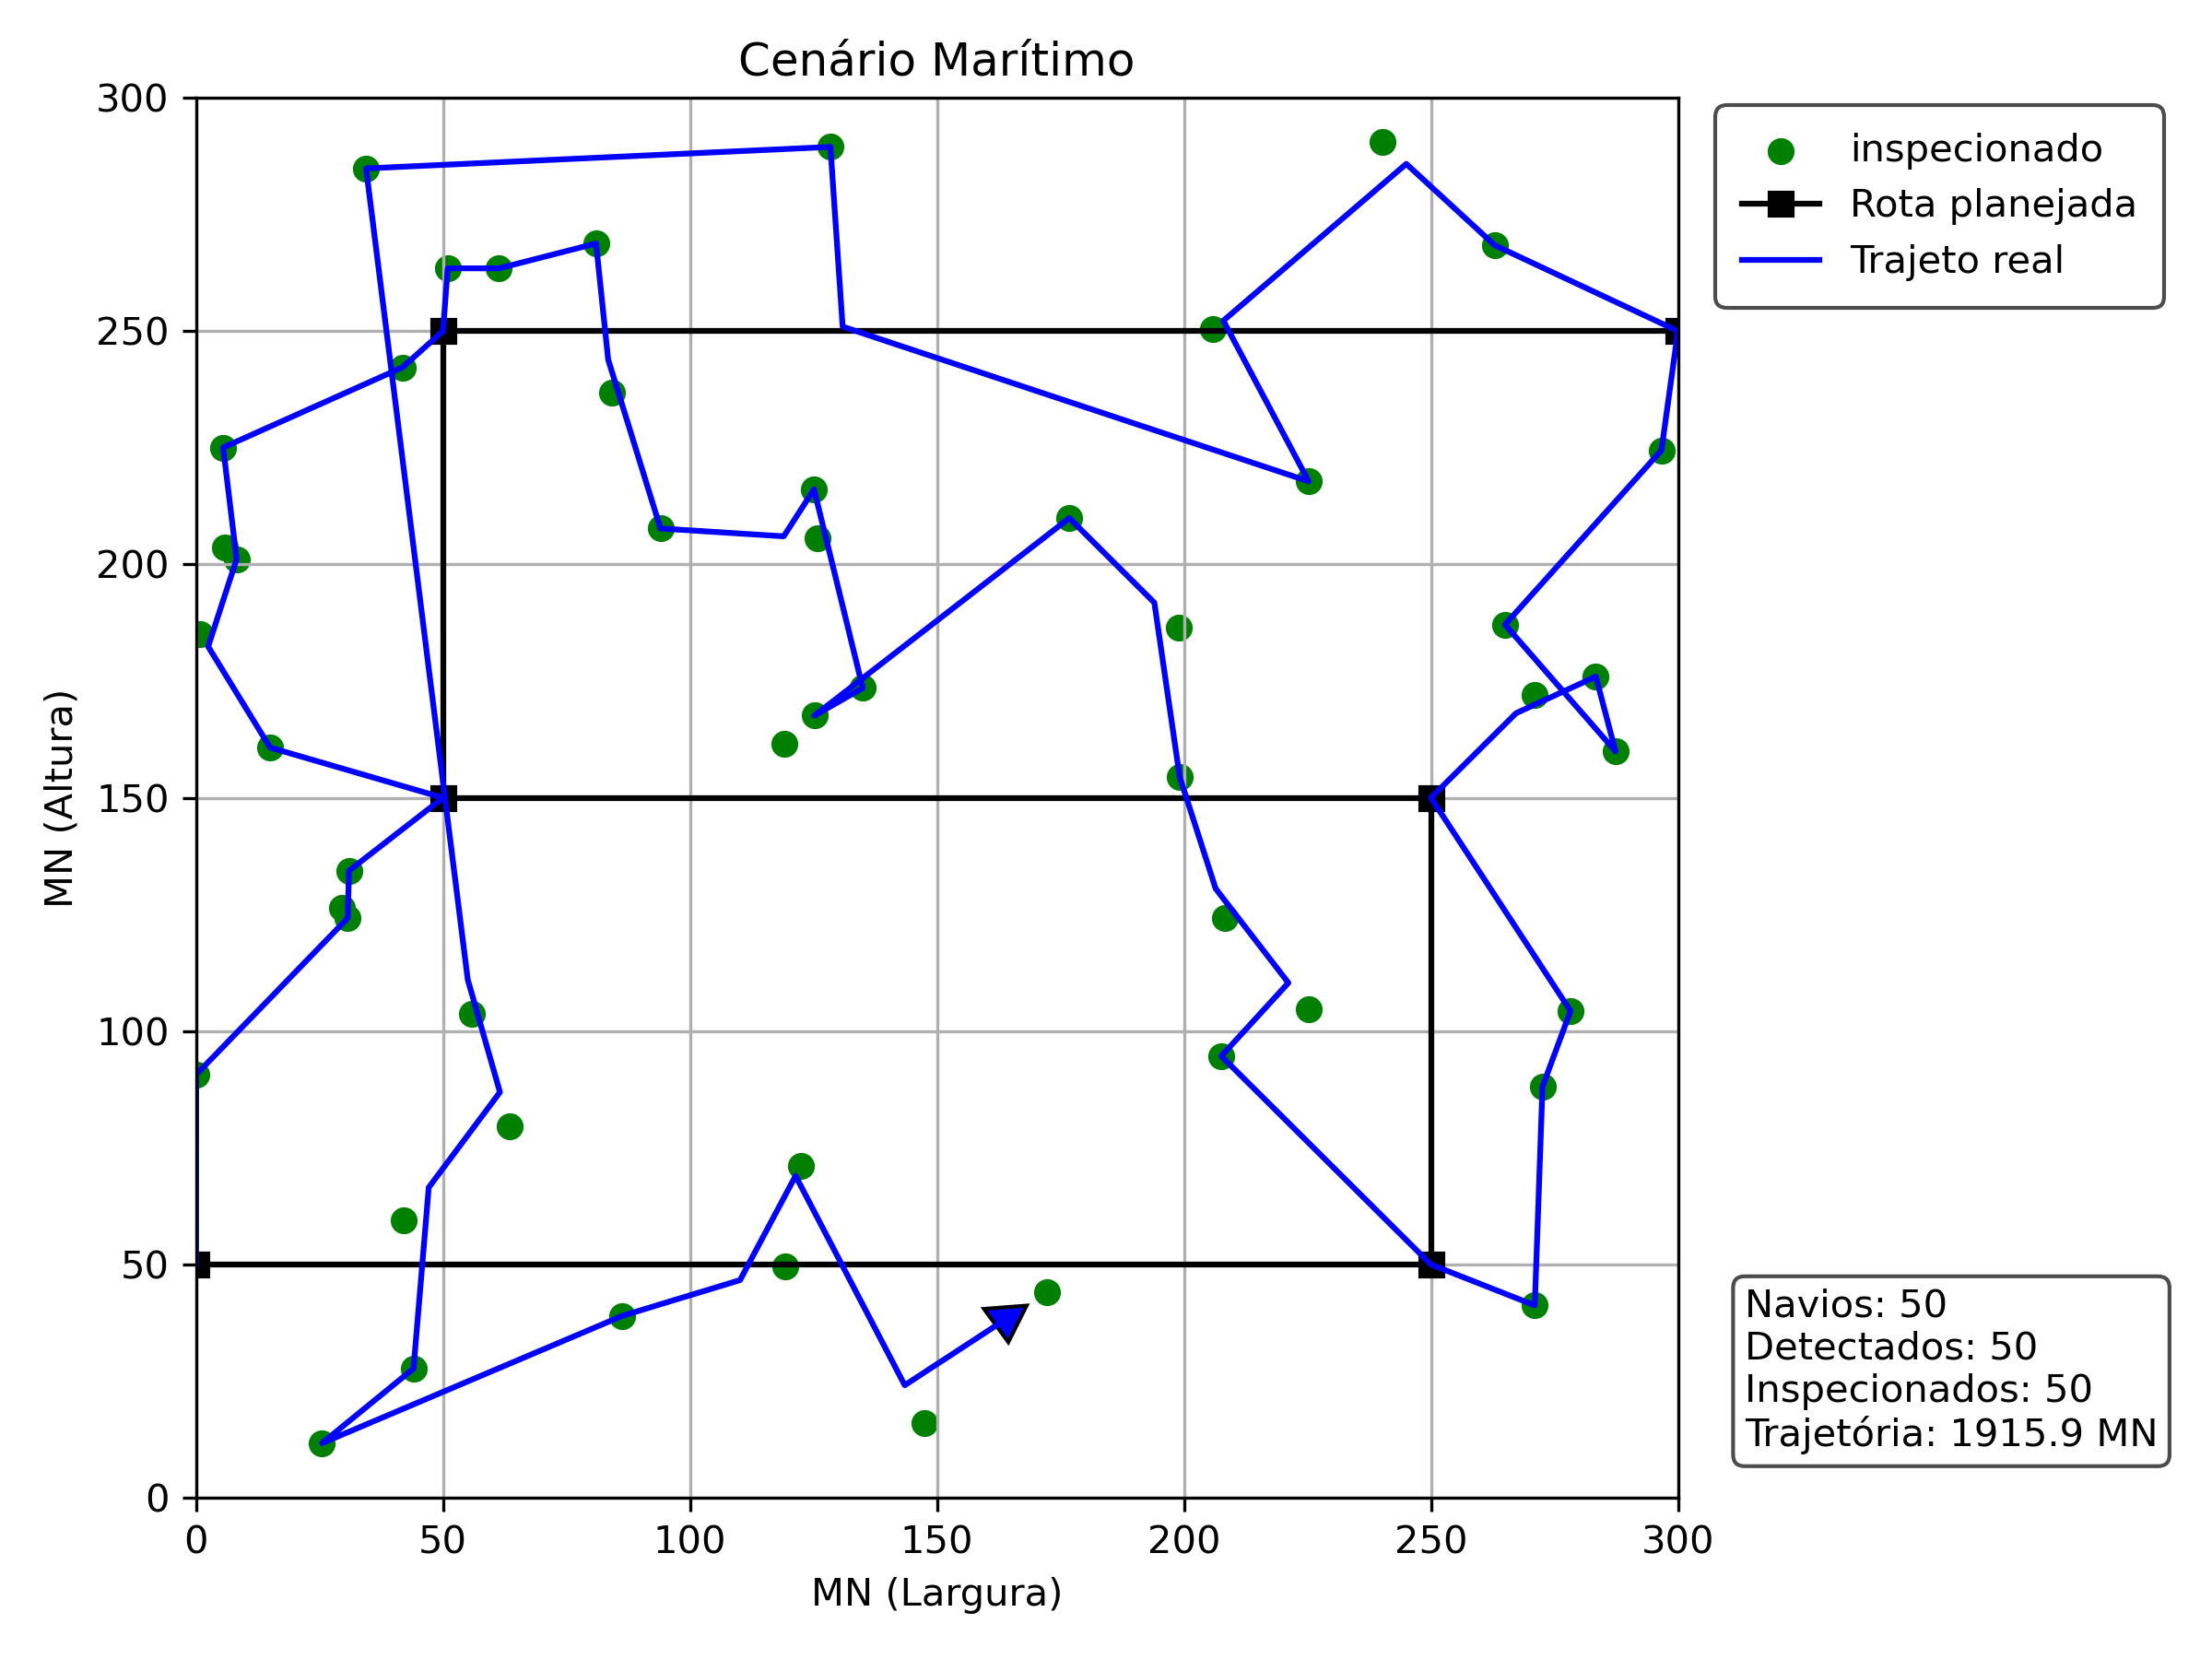
\includegraphics[width=\linewidth]{fig/greed.png}
        \caption{\textit{Greed}}
        \label{fig:trajetoria_greed}
    \end{subfigure}
    \hfill
    \begin{subfigure}{0.4\textwidth}
        \centering
        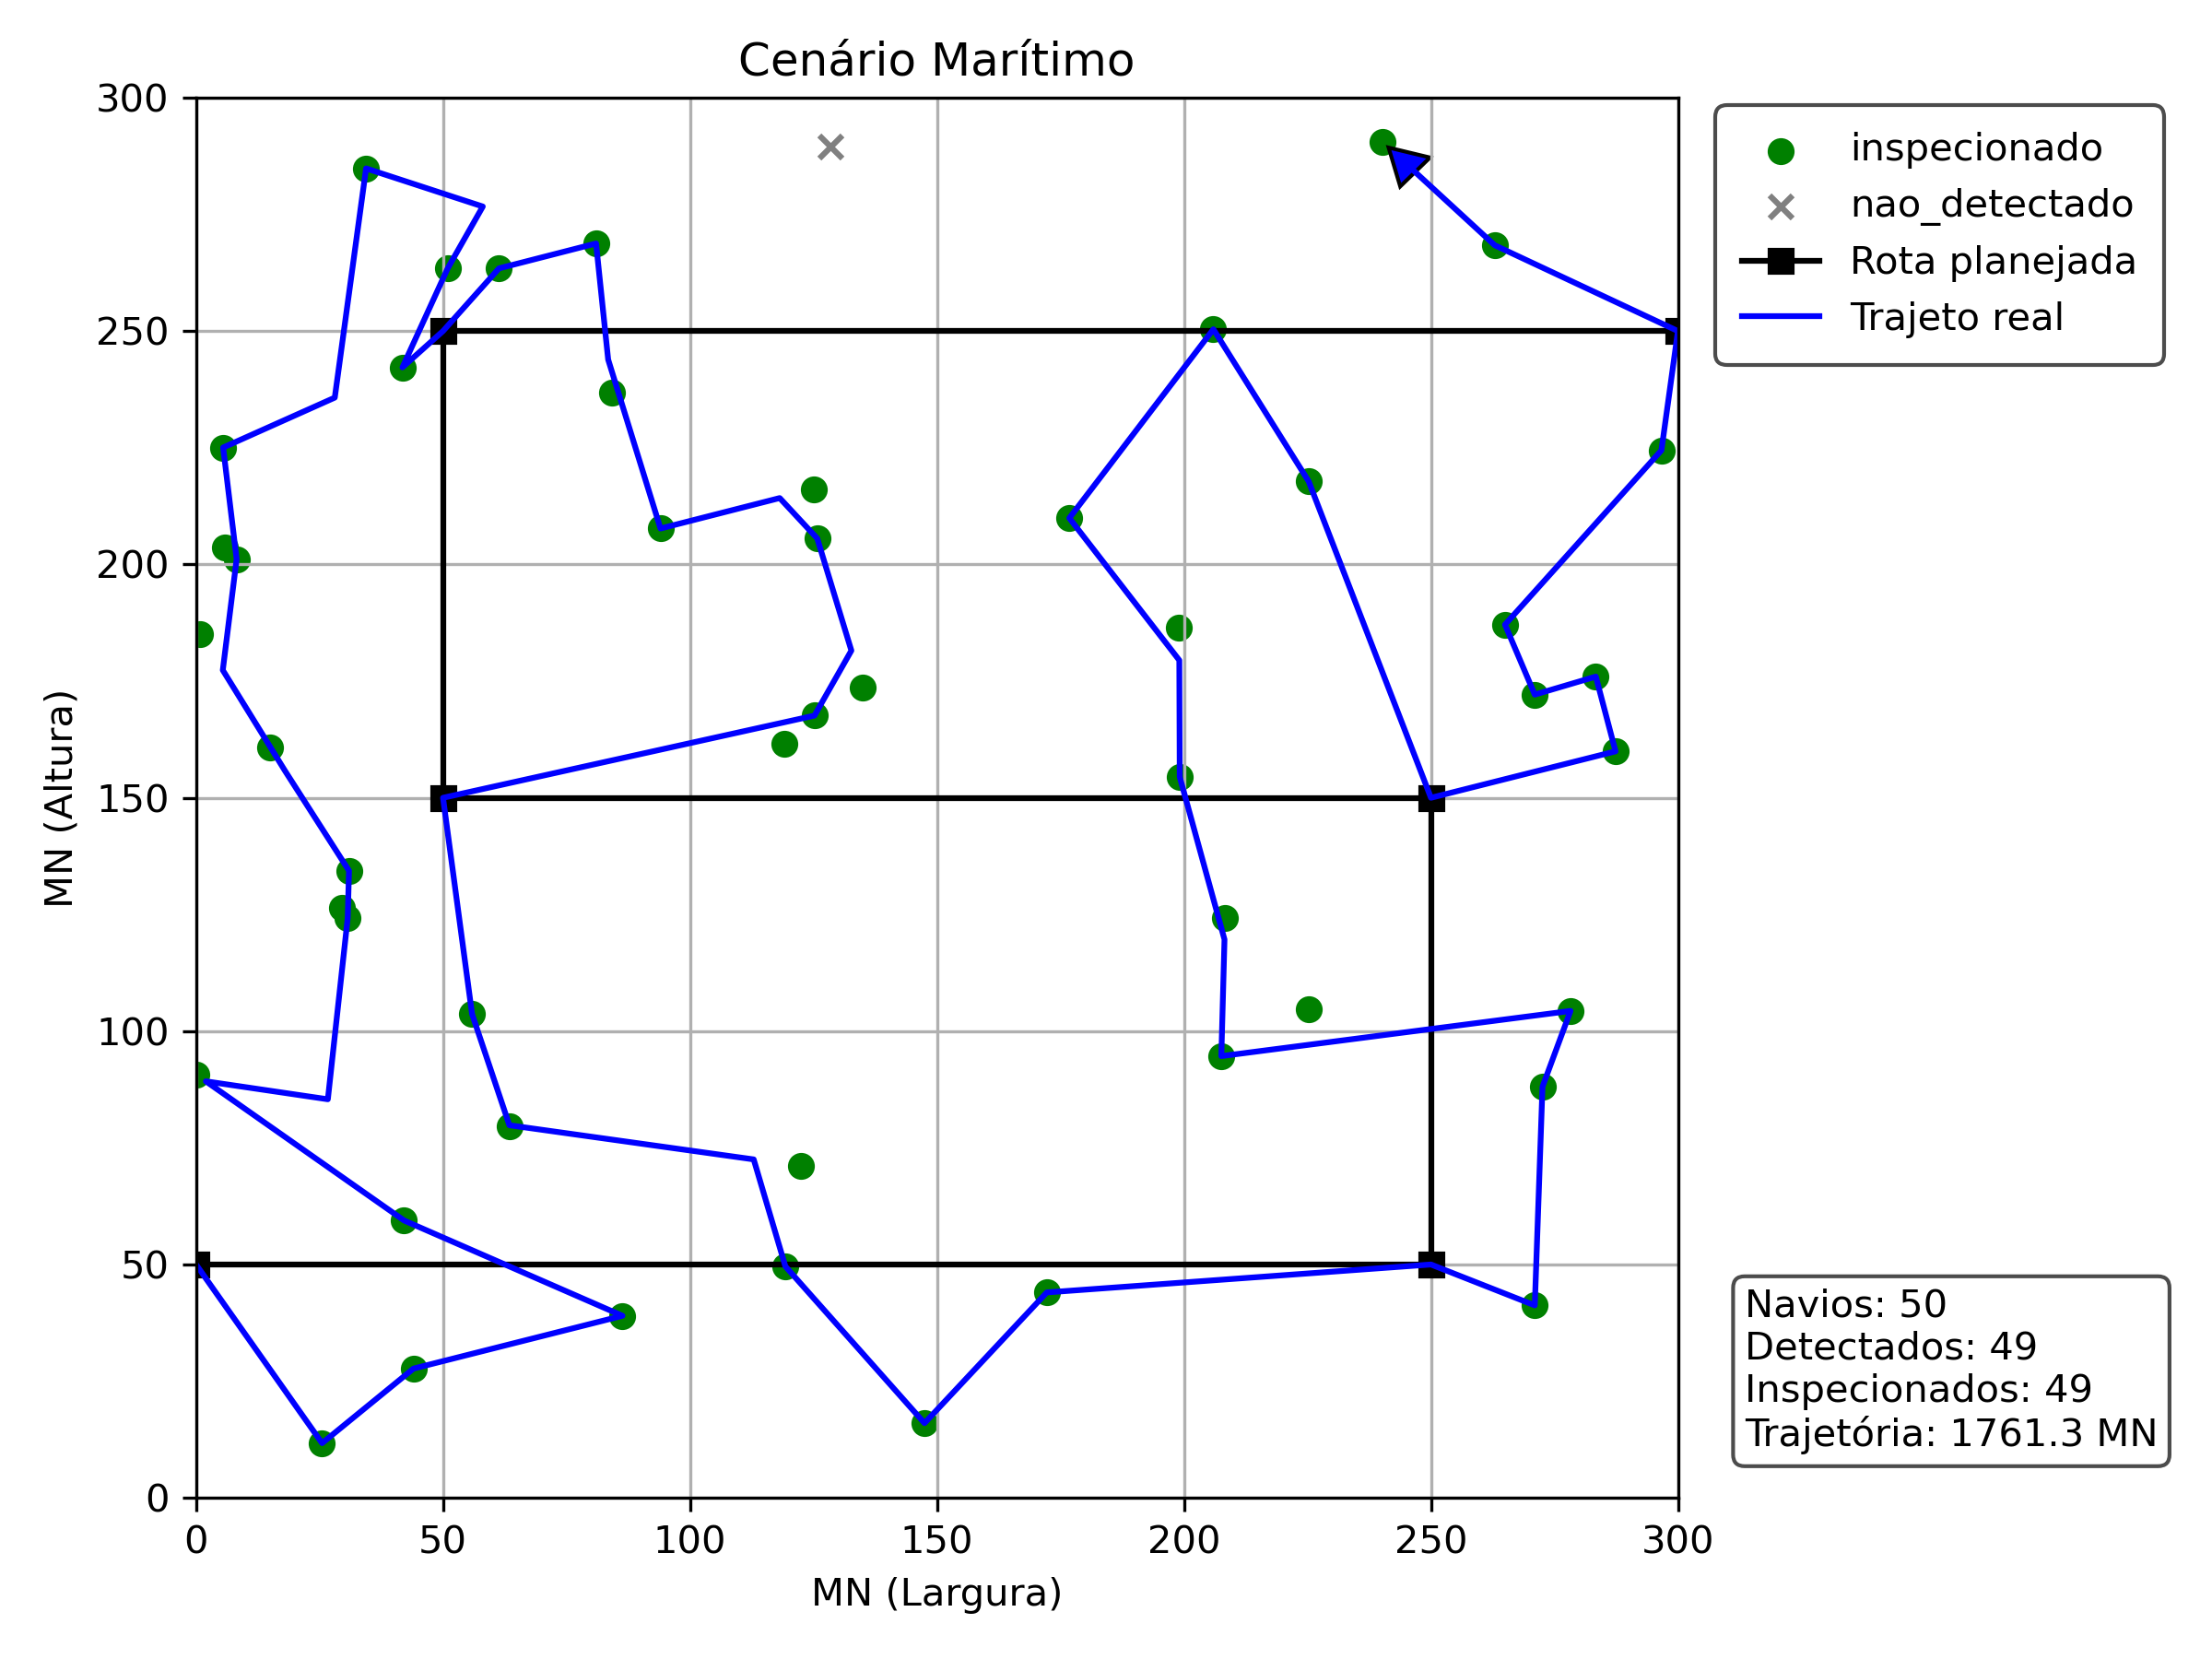
\includegraphics[width=\linewidth]{fig/SA.png}
        \caption{\textit{Simulated Annealing}}
        \label{fig:trajetoria_sa}
    \end{subfigure}
    \caption{Trajetória do VANT para as três políticas de navegação (50 navios).}
    \label{fig:trajetorias_comparacao}
\end{figure}

Na política \textit{passiva}, o VANT segue rigorosamente a rota de referência. Na \textit{greed}, ele desvia para inspecionar os alvos mais próximos, resultando em uma trajetória mais adaptativa, porém com sobreposição de caminhos. Já na \textit{Simulated Annealing}, a rota também é ajustada, mas de forma mais otimizada, minimizando a distância e evitando cruzamentos. Isso indica maior eficiência da política estocástica em termos de percurso.
